\documentclass[10pt,a4paper]{article}

\usepackage[utf8]{inputenc}
\usepackage[T1]{fontenc}
\usepackage{mathptmx}
\usepackage[margin=1.25cm,top=1.1cm,bottom=1.15cm]{geometry}
\usepackage{xcolor}
\usepackage{graphicx}
\usepackage{hyperref}
\usepackage{enumitem}
\usepackage{titlesec}
\usepackage{array}

\definecolor{cvblue}{HTML}{0875D1}
\hypersetup{
  colorlinks=true,
  urlcolor=cvblue,
  linkcolor=cvblue
}

\pagestyle{empty}
\setlength{\parindent}{0pt}
\setlength{\parskip}{0pt}
\setlist[itemize]{leftmargin=1.15em,itemsep=1pt,topsep=1pt,parsep=0pt}
\setlist[itemize,2]{label={-},leftmargin=1.5em,itemsep=1pt,topsep=0.5pt}
\titleformat{\section}
  {\color{cvblue}\Large\bfseries}
  {}
  {0pt}
  {}
  [\color{cvblue}\titlerule]
\titlespacing*{\section}{0pt}{5pt}{3pt}

\newcommand{\cvright}[1]{\hfill{\normalfont #1}}
\newcommand{\cvrole}[3]{%
  \item \textbf{#1:} #2 \cvright{#3}
}
\newcommand{\cvproject}[3]{%
  \item \textbf{#1} #2 \cvright{#3}
}
\newcommand{\cvedu}[4]{%
  \item \textbf{#1:} #2 \cvright{#3}\\
  \textit{Focus: #4}
}

\begin{document}
\small

\begin{minipage}[t]{0.82\textwidth}
  \centering
  {\Huge\bfseries\color{cvblue} Zeyu Wang}\\[4pt]
  Berlin, Germany \quad | \quad +49 170 6991380 \quad | \quad \href{mailto:wzy07777@gmail.com}{wzy07777@gmail.com}\\
  Date of Birth: 30.06.2003 \quad | \quad JiangSu Province, China\\
  LinkedIn: \href{https://www.linkedin.com/in/wang-zeyu-72b214395}{wang-zeyu-72b214395}
\end{minipage}
\begin{minipage}[t]{0.17\textwidth}
  \raggedleft
  % Upload zeyu_photo.png to the same Overleaf project folder.
  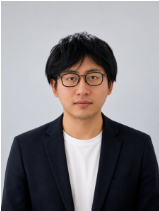
\includegraphics[width=1.9cm,height=2.55cm,keepaspectratio]{zeyu_photo.png}
\end{minipage}

\section*{Profile}
M.Sc. Computer Science student at TU Berlin and CKA/CKS-certified cloud engineer focused on Linux infrastructure, container orchestration, production automation and agent-facing backend tools. Hands-on experience with Go services, Docker, Kubernetes, AWS/GCP deployment assets, RAG workflows, fine-tuning data pipelines and cloud operations.

\section*{Skills}
\begin{itemize}
  \item \textbf{Cloud Platforms:} AWS EC2/RDS, Google Cloud Platform, Cloudflare R2
  \item \textbf{Containers / IaC:} Docker, Docker Compose, Kubernetes, Ansible, Terraform, Caddy
  \item \textbf{Backend / Data:} Go/Gin, GraphQL, MCP, PostgreSQL/PostGIS, Redis, JWT/RBAC, OAuth, REST APIs
  \item \textbf{AI / Agents:} \textbf{RAG}, \textbf{fine-tuning data preparation}, embeddings, hybrid retrieval, ReAct/ReactAgent, NetworkX
  \item \textbf{Programming:} Go, Python, TypeScript; basic Java
\end{itemize}

\section*{Certifications}
\begin{itemize}
  \item \textbf{CKA:} Certified Kubernetes Administrator \cvright{The Linux Foundation}
  \item \textbf{CKS:} Certified Kubernetes Security Specialist \cvright{The Linux Foundation}
\end{itemize}

\section*{Work Experience}
\begin{itemize}
  \cvrole{03.2024 - 06.2024}{AI / Backend Engineer Intern, Part-time}{JH UniScheduler / Jhinno}
    \begin{itemize}
      \item Worked on \textbf{RAG} and \textbf{fine-tuning} workflows for Jiaozi/Dumpling, turning user model requirements and dataset metadata into structured retrieval and generation tasks.
      \item Built retrieval components with \textbf{Python}, embeddings, graph knowledge-base metadata, hybrid scoring and prompt templates to support model selection and code generation.
      \item Developed \textbf{Golang} service modules and supported \textbf{Docker} / \textbf{Kubernetes} development, testing and deployment workflows for AI/backend components.
      \item Prepared fine-tuning and evaluation datasets from generated training-code traces, failure cases and self-correction logs for a \textbf{multi-agent AutoDL pipeline}.
    \end{itemize}
\end{itemize}

\section*{Projects}
\begin{itemize}
  \cvproject{03.2026 - Present:}{WeJoin - Cloud-Native Campus Platform}{\href{https://wejoin.store}{wejoin.store}}
    \begin{itemize}
      \item \textbf{Tech Stack:} \textbf{Go/Gin}, React, TypeScript, PostgreSQL/PostGIS, Redis, Cloudflare R2, Docker Compose, Caddy, Terraform, Ansible.
      \item Built a modular campus platform for map-based events, course reviews and moderation with a Go/Gin API and React/TypeScript frontend.
      \item Containerized with Docker Compose and Caddy; integrated PostgreSQL/PostGIS, Redis, Cloudflare R2, tracked migrations, health checks and recovery runbooks.
    \end{itemize}

  \cvproject{06.2026 - Present:}{MiSArch Agent Gateway - MCP / A2A for Microservices}{Go, MCP, GCP}
    \begin{itemize}
      \item \textbf{Tech Stack:} \textbf{Go}, MCP, GraphQL, ReactAgent, A2A, Docker Compose, Google Cloud Platform, Python evaluation scripts.
      \item Built a \textbf{Go MCP gateway} over MiSArch GraphQL to expose catalog lookup and pending-order workflows as agent-facing tools with typed input schemas.
      \item Designed an \textbf{agent interoperability} architecture with a user-side private assistant agent and company-side service agents, enabling flexible \textbf{A2A} integration across different service providers.
      \item Planned personalized recommendation and requirement-adaptation flows where the private agent adjusts requests based on user habits, then negotiates with service agents through MCP tools, GraphQL access or direct multi-agent collaboration.
      \item Deployed the MiSArch stack and gateway on \textbf{GCP} with Docker Compose; compared raw GraphQL, MCP tool access and agent-oriented interaction paths in repeatable smoke tests and A/B-style evaluations.
    \end{itemize}

  \item \textbf{Dumpling, an End-to-End AutoDL agent}
    \begin{itemize}
      \item \textbf{Tech Stack:} \textbf{Python}, RAG, fine-tuning data preparation, ReAct, NetworkX DiGraph, embeddings, hybrid retrieval, multi-agent orchestration.
      \item Organized and led a 6-person team as initiator and architect to build an agent-based automated deep learning platform.
      \item Designed a graph-based model knowledge base with 14 backbones and 22 checkpoints, typed edge semantics and hybrid retrieval scoring.
      \item Designed a ReAct-based self-correction mechanism for multi-agent autonomous error correction and ablation experiments on generated code.
    \end{itemize}
\end{itemize}

\section*{Education}
\begin{itemize}
  \cvedu{10.2025 - 07.2027}{Computer Science, M.Sc.}{Technical University Berlin}{Cloud Infrastructure, Kubernetes, Docker, Ansible, AI Agent}
  \cvedu{09.2021 - 06.2025}{Computer Software Engineering, Bachelor}{Xidian University}{Computer Science, Software Engineering, Go Development}
\end{itemize}

\section*{Languages}
\begin{itemize}
  \item Chinese \cvright{Native}
  \item German \cvright{B2}
  \item English \cvright{C1}
\end{itemize}

\end{document}
